\documentclass[11pt]{article}
\usepackage[margin=1in]{geometry}
\usepackage{amsmath,amssymb,amsthm,graphicx,booktabs,hyperref}
\newtheorem{proposition}{Proposition}
\title{Memory, History Access, and Parallel Refinement\\\large Exact MVP and Frozen-Model Competence Study}
\author{Exploratory research note}
\date{September 21, 2026}
\begin{document}
\maketitle
\begin{abstract}
We distinguish limited retained information, renewed access to history, and dependence missed by independent parallel output heads. Exact experiments verify restricted scan-cost identities, finite binary compression optima, and the effect of representation structure on parallel sampling. All 35 rank-two encoders on four bits retain the same information, but their one-round forward KL errors range from zero to two bits. An information-set construction is exact in two rounds under a restricted coordinate-reveal interface. These are explanatory results with classical ingredients, not a new general theorem for RWKV or diffusion. A separate frozen-model pilot tests competence before further empirical expansion.
\end{abstract}
\section{Access and memory contracts}
A bounded-state decoder receives an encoding formed before the query, then computes without rereading history. A history-access decoder may rescan the original records. Persistent canvases, scratch tokens, caches, indices and finite-precision states must count toward any claimed memory bound. The GPU cap is 32 queued or running H100s, eight per job. The pilot uses existing frozen models without pretraining and does not replace earlier E3 confirmation.

For $M$ independent uniform $V$-ary records, a uniform query revealed after a $B$-bit encoding satisfies the standard converse
\[
 H(Y\mid C,Q)\ge\max\{0,\log_2V-B/M\}.
\]
Indeed, $H(X\mid C)\ge M\log_2V-B$; conditional subadditivity and averaging over queries prove the inequality. Fano then constrains error irrespective of decoder iterations. Exact codebook enumeration shows why retaining whole records is not always optimal: with three source bits and one memory bit, optimal random-query accuracy is 75\%, versus 66.7\% for storing one source bit. This is a standard coding result, not new theory.

\section{Restricted history scans}
An online walker follows a chain of $h$ unique key/value records. It retains its current key, cannot cache off-path records, and advances only when it encounters the active key. A scan is one directional traversal. If $p_i$ is the position of the $i$th required edge, forward scans cost $1+\operatorname{des}(p)$. Each increasing run is consumed in one scan; every descent requires restarting. For uniform record order the distribution is Eulerian and the mean is $(h+1)/2$.

Alternating directions starting forward cost one plus the initial direction mismatch plus subsequent direction changes. Their mean is $(4h+1)/6$ for $h\ge2$: the first mismatch has probability $1/2$, and each subsequent sign change has probability $2/3$. This is a classical longest-alternating-subsequence statistic \cite{stanley}. It is not a general neural streaming lower bound.

Independent simulation follows opaque key/value records and verifies all 46,233 permutations through eight hops, with zero mismatches. At eight hops, forward scans average 4.5 and alternating scans 5.5. Reverse-ordered chains instead need $h$ forward scans and two alternating scans. A single off-path cached record invalidates the no-cache bound, as the explicit control demonstrates.
\begin{figure}[ht]
\centering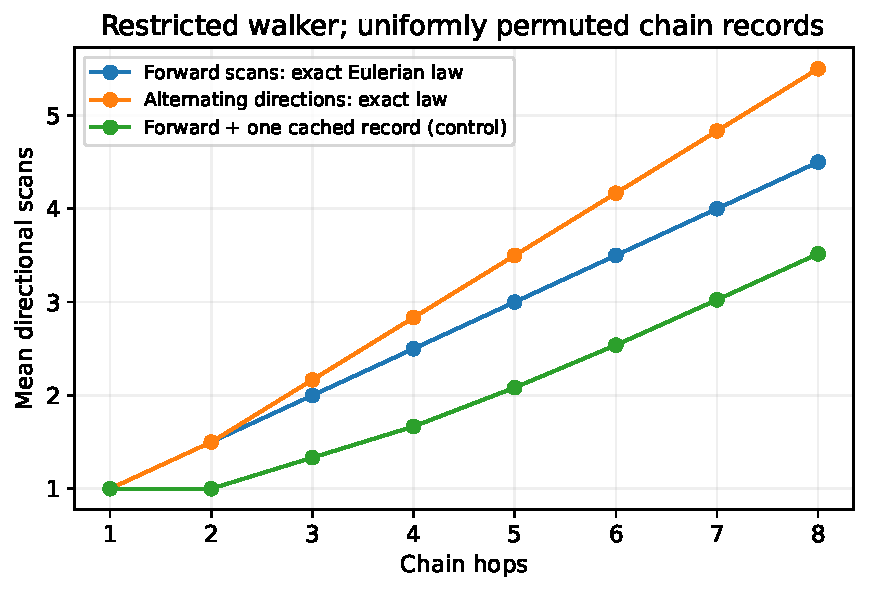
\includegraphics[width=.8\linewidth]{../results/theory_mvp/scan_cost.pdf}
\caption{Exact restricted-walker experiment. Directions are charged as separate scans. The FIFO-cache control is a different algorithm.}
\end{figure}

\section{Equal information, different parallel error}
Let $Y=H$ be uniform on $\mathbb F_2^N$, with compression $C=AH$, $\operatorname{rank}(A)=r$. Let $d(A)$ count coordinate unit vectors in the rowspace of $A$.
\begin{proposition}
All rank-$r$ encoders retain $r$ bits. Sampling exact coordinate posterior marginals independently nevertheless yields
\[
D_{\rm KL}\!\left(p(Y\mid C)\middle\Vert\prod_i p(Y_i\mid C)\right)=(r-d(A))\ln2,
\quad \mathrm{TV}=1-2^{-(r-d(A))}.
\]
\end{proposition}
\begin{proof}
The posterior is uniform on an affine space of size $2^{N-r}$. A coordinate is fixed iff its unit vector is in the rowspace; otherwise it is fair. The product is uniform on a containing coordinate subcube of size $2^{N-d}$. Its constant likelihood ratio on the true support gives KL; the shared probability mass gives TV.
\end{proof}
Full-history expected log loss is $(N-d)\ln2$, the sum of compression loss $(N-r)\ln2$ and the product-posterior gap. These quantities must not be conflated.

After some coordinates are observed, let $U$ be the unknown set and $J\subseteq U$ a batch. Let $d_{U,J}$ count individually fixed coordinates in $J$. Projection of the affine posterior gives
\[
\operatorname{TC}(Y_J\mid C,Y_{U^c})=
[\operatorname{rank}(A_U)-\operatorname{rank}(A_{U\setminus J})-d_{U,J}]\ln2.
\]
The projected entropy is $[|J|-\operatorname{rank}(A_U)+\operatorname{rank}(A_{U\setminus J})]\ln2$; subtract it from the sum of coordinate entropies.

Choose a coordinate information set of size $N-r$ for the nullspace code. These posterior bits are independent and fair. Sample them in one batch, then solve and reveal the remaining deterministic coordinates. One batch is exact iff $r=d(A)$; otherwise two are sufficient and necessary \emph{only for irreversible original-coordinate reveals with independent within-batch draws}. Shared latent randomness and a linear output map can sample the code in one computation. Solving cost, matrix storage and exact conditional access are not free recurrent capabilities.

\begin{table}[ht]\centering
\begin{tabular}{rrr}\toprule
One-round KL (bits)&Encoders&Constraint satisfaction\\\midrule
0&6&100\%\\1&16&50\%\\2&13&25\%\\\bottomrule
\end{tabular}
\caption{All 35 rank-two rowspaces on four bits. Each retains two bits and leaves two bits of conditional entropy. The two-round construction is exact for every encoder.}
\end{table}
All compression values and feasible partial observations give 24,592 batch-dependence identities, checked with zero residual. An additional six-bit encoder with rows 001111 and 110011 has all 15 pairs conditionally independent, but global total correlation two bits and product-law constraint satisfaction 25\%. Pairwise screening alone therefore cannot certify a product joint. This does not establish a failure of any named sampler without checking its actual tests.
\begin{figure}[ht]\centering
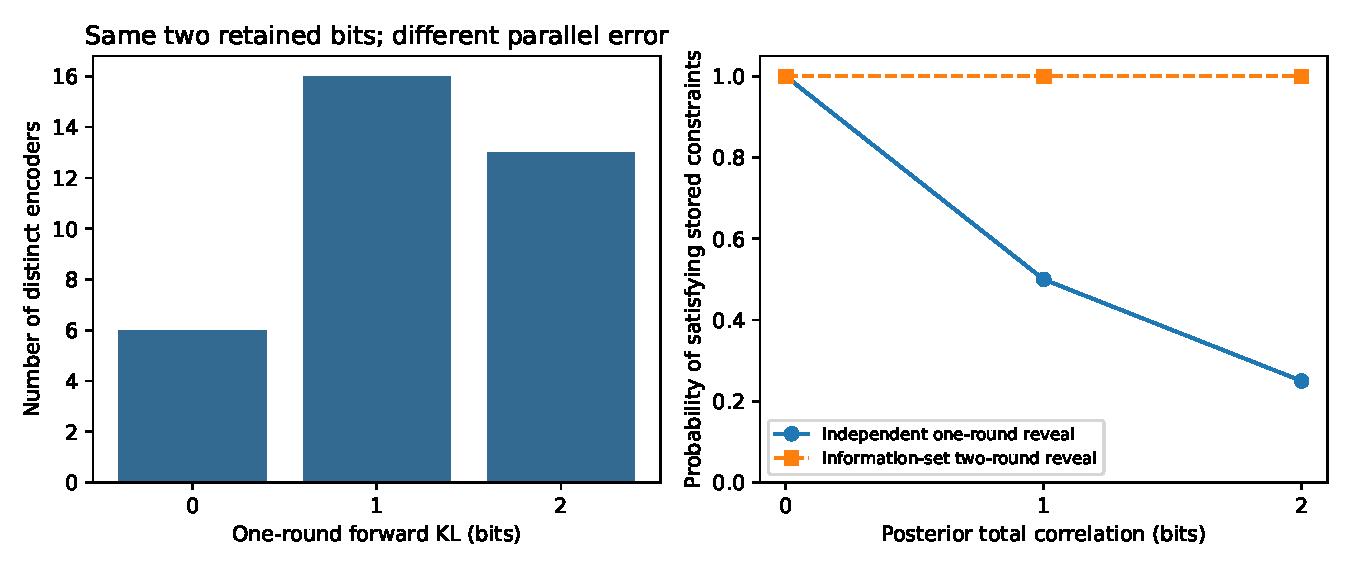
\includegraphics[width=\linewidth]{../results/theory_mvp/representation_parallelism.pdf}
\caption{Exact oracle systems at fixed retained information, not measurements of learned F2 states.}
\end{figure}

\section{Exact absorbing-schedule experiment}
An exact dynamic program evaluates independent absorbing reveals at 1, 2, 4, 8, 16, 32, 64 and 128 stages for each of the 35 encoders. It tracks both surviving feasible partial assignments and the expected path dependence cost. Once irreversible commitments make a projected constraint infeasible, no completion can enter the true support. Affine symmetry then gives endpoint forward KL of $-\log_2$ of the valid-support probability.

For two independent parity pairs, a pair's reveal stages coincide with probability $1/T$. Endpoint constraint satisfaction is therefore $(1-1/(2T))^2$, and expected path dependence is $2/T$ bits. At 1, 8 and 64 stages, endpoint KL is respectively 2, 0.186219 and 0.022631 bits; the path bounds are 2, 0.25 and 0.03125 bits. The information-set two-round construction is exact, while a systematic encoder is exact in one round. These are oracle schedule comparisons, not measured neural speedups.
\begin{figure}[ht]\centering
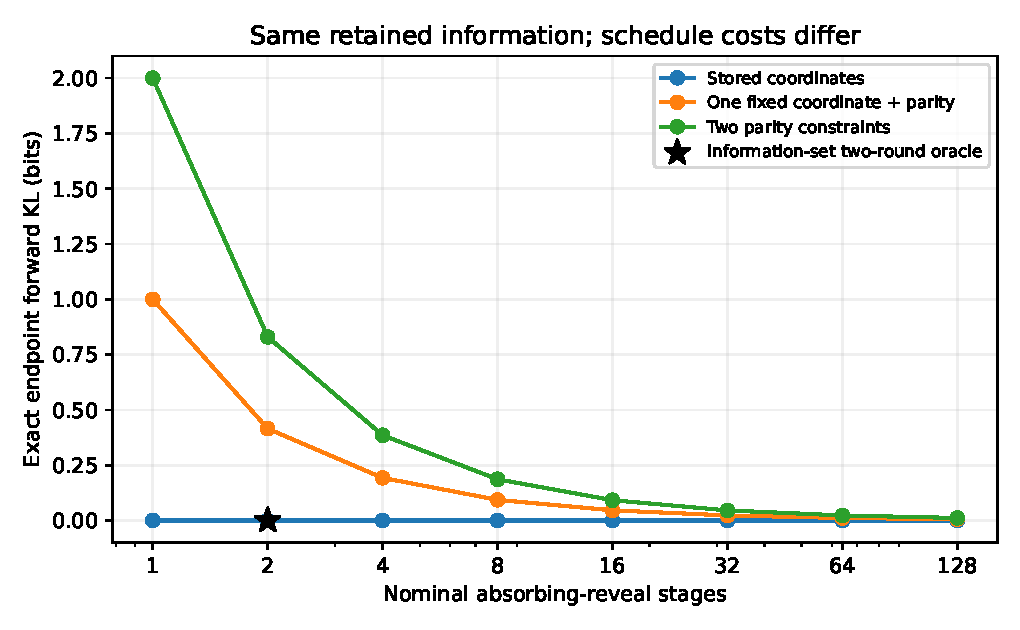
\includegraphics[width=.78\linewidth]{../results/theory_mvp/reveal_schedule.pdf}
\caption{Exact schedule comparison at equal retained information. Stages count nominal independent-reveal rounds, not GPU cost.}
\end{figure}

\section{Frozen-model competence pilot}
Each model receives the same 120 one-hop and 120 two-hop natural-language lookup examples, balanced across 24 colors. One fixed instruction requests a color on the first line. Both models receive a 32-token output budget, not gold answer length. F2 uses eight matched-Bernoulli stages at temperature 0.7; causal RWKV uses greedy decoding. The frozen first-line parser determines the gate; full-output whole-word reference occurrence is a separate diagnostic.

Each model must score at least 96/120 at each depth, with complete coverage and provenance, before paired long-context expansion is allowed. The prompts contain no long neutral filler. This tests interface competence, not the binary-code theorem.
\IfFileExists{../results/theory_mvp/pilot_table.tex}{\begin{table}[ht]\centering\small
\begin{tabular}{llrrr}\toprule
Model & Depth & Exact / 120 & 95\% Wilson interval & Gold anywhere / 120\\\midrule
F2 & 1-hop & 22 (18.3\%) & [12.4,26.2]\% & 57\\
F2 & 2-hop & 1 (0.8\%) & [0.1,4.6]\% & 14\\
R0 & 1-hop & 63 (52.5\%) & [43.6,61.2]\% & 110\\
R0 & 2-hop & 29 (24.2\%) & [17.4,32.6]\% & 32\\
\bottomrule\end{tabular}
\caption{All 480 audited pilot outputs. Every cell fails the frozen 96/120 competence threshold. Wilson intervals are descriptive for fixed balanced development tasks, not multiplicity-adjusted confirmation. Gold occurrence is a separate diagnostic and can include ambiguous continuations.}
\end{table}
\paragraph{Gate decision.} No long-context expansion. One-hop inputs contain 121--129 native tokens; two-hop inputs contain 209--219. F2 produces 36 and 17 parseable first-line answers; R0 produces 71 and 103. Although R0 mentions the reference color in 110/120 one-hop outputs, this diagnostic does not change the frozen gate. In F2 one-hop outputs, 31 of the 57 reference-containing continuations also mention another candidate color. Two-hop failure persists even with the permissive occurrence diagnostic.
\paragraph{Runtime scope.} The job uses the recorded FLA implementation, whose warning recommends checking against the official RWKV implementation. Artifact and tokenizer checks do not establish independent official-kernel parity. These are observations of the qualified frozen-model runtime and task interface, not a general impossibility claim about the checkpoints.
\paragraph{Resources.} One eight-H100 job succeeded with 316 seconds of scheduler-reported running time (approximately 0.70 H100-hours, not a billing estimate). The concurrency cap remained 32; no further jobs were launched.
}{The pilot is pending collection; no competence claim is made yet.}

\section{Decision and novelty limits}
The scan identities, coding bounds and linear-code constructions have classical ingredients \cite{stanley,reing}. Conditional-independence sampling and dependence-based serial depth are also established research directions \cite{punt,wen}. The MVP does not establish a new general theorem or a long-context advantage for recurrent diffusion. A stronger contribution needs a new certified method or sharp tradeoff for approximate recurrent representations under explicit storage and computation limits, plus a qualified implementation testing its predictions.

Original deterministic full-history lookup tasks have point-mass answer posteriors and zero true conditional total correlation. They cannot validate a positive dependence penalty. The exact compressed-code study deliberately supplies nontrivial posterior dependence; it and the model pilot are different systems.

\begin{thebibliography}{9}
\bibitem{stanley} R. Stanley. Longest alternating subsequences of permutations. \url{https://arxiv.org/abs/math/0511419}.
\bibitem{reing} K. Reing et al. Maximizing Multivariate Information with Error-Correcting Codes. \url{https://arxiv.org/abs/1811.10839}.
\bibitem{punt} I. Azangulov et al. Parallel Sampling from Masked Diffusion Models via Conditional Independence Testing. \url{https://arxiv.org/abs/2510.21961}.
\bibitem{wen} C. Wen et al. Conditional Total Correlation and the Serial Depth of Adaptive Parallel Sampling. \url{https://arxiv.org/abs/2608.25505}.
\end{thebibliography}
\end{document}
